% ----------------------------------------
% Chap: Konstruktive Bearbeitung
% ----------------------------------------
\chapter{Konstruktive Bearbeitung}
\label{chap:konstruktive_bearbeitung}

Um die Messgenauigkeit der optischen Interferometrie-Technik mit der einfachen Adaptierbarkeit an verschiedenen realen Maschinenelementen der elektrischen Messmethode zur Schmierfilmdickenmessung im EHD-Kontakt zu vereinigen, soll ein neues modular Messsystem auf Basis des EHD-Prüfstands von PCS entwickelt werden.
Dies System soll die optische und elektrische (kapazitive) Messung gleichzeitig erlauben.
Für solches System gibt es die folgende Anforderungen, die durch konstruktive Bearbeitung in nächsten Abschnitten gelöst werden.
\begin{itemize}
    \item Elektrische Isolierung der Glasscheibe und der Kugel mit dem gesamten System.
    \item Elektrische Zugänge für die Messproben an der Scheibe und der Kugel.
    \item Beschichtung auf der Scheibe, die elektrische und optische Messung gleichzeitig erlaubt.
\end{itemize}

% ----------------------------------------
% Sec: Konstruktion der Kugelführung
% ----------------------------------------
\section{Konstruktion der Kugelführung}
\label{sec:konstruktion_der_kugelfuehrung}

Da das modifizierte Kugelsupport mit einstellbarer Achse von \textit{E. Wittek} \cite{wittek_2007} wegen Rundlaufabweichung nur bis Wälzgeschwindigkeit von c.a 0,7 $m/s$ einsetzbar ist, wird die originale Kugelführung der PCS Firma im Rahmen dieser Arbeit modifizierte und weiter benutzt.
Bei der standardmäßigen Kugelführung wird eine durchgebohrte Kugel in einem Adapter eingeklemmt, welche dann über einen Querstift mit der Motorausgangswelle des zweiten Antriebs formschlüssig verbunden wird.
Für die kapazitive Messung soll die Kugel elektrisch mit dem gesamten System isoliert werden, das erfolgt durch die Verwendung eine Kunststoffwelle.
Die Kugelaufnahme wird aus Messing gefertigt, um den Kontaktwiderstand mit den zu Signal übertragenden Kohlebürsten zu reduzieren.
Die Abbildung \ref{fig:aufbau_der_neuen_kugelfuehrung} zeigt den Zusammenbau der neuen Kugelführung.
% ----------------------------------------
% Fig: Aufbau der neuen Kugelführung
% ----------------------------------------
\begin{figure}[htb]
    \centering
    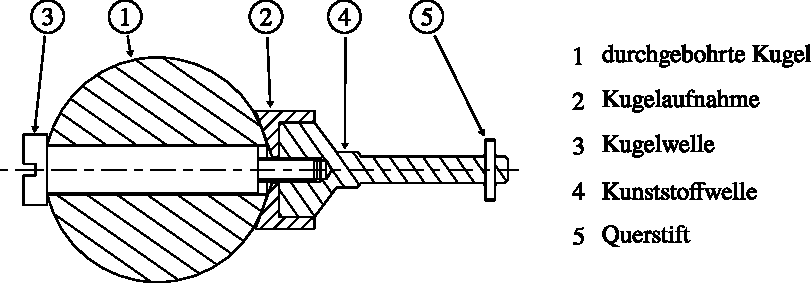
\includegraphics[]{./images/durchgebohrte_kugel.pdf}
    \caption{Aufbau der neuen Kugelführung}
    \label{fig:aufbau_der_neuen_kugelfuehrung}
\end{figure}
%

Die geführte Kugelachse ermöglicht die Versuche mit Schlupf und verhindert auch das unkontrollierte Einbringen des Schmierstoffes (Öl, Fett) in den Kontakt.
Der Kraftfluss zwischen dem zweiten Motor und der Kugel kann durch den Wegfall des Querstifts unterbrochen werden.
In diesem Fall dreht sich die Kugelführung frei in der Motorausgangswelle.

% ----------------------------------------
% Sec: Konstruktion des Kugelsupports
% ----------------------------------------
\section{Konstruktion des Kugelsupports}
\label{sec:konstruktion_des_kugelsupports}

Das neue Kugelsupport besteht aus drei Rillenkugellager, die durch drei $M3$ Schrauben auf einem dreieckigen Sockel befestigt werden (Abbildung \ref{fig:das_modifizierte_kugelsupport}).
Die Kugel wird von den drei Lagern sicher von unten gegen der Glasscheibe gestützt.
Da die Kugel mit der Lasteinheit elektrisch isoliert werden muss, wird der Sockel aus Kunststoff gefertigt.
Auf der Unterseite des Sockels befinden sich zwei Löcher, die mit den Stifte der Lasteinheit arretiert werden, dadurch wird die Position des Kugelsupports während Versuche sicher gestellt.
An der Seite des Sockels sind zwei M3 Bohrung zur Anbringung der Kohlebürstenhalter, die für die Aufnahme der elektrischen Signale von der Kugel zuständig sind, zu versehen.
Bei der Versuchen mit Fett ist dort auch möglich, die Befettungsvorrichtung zu montieren.
% ----------------------------------------
% Fig: Das modifizierte Kugelsupport
% ----------------------------------------
\begin{figure}[htb]
    \centering
    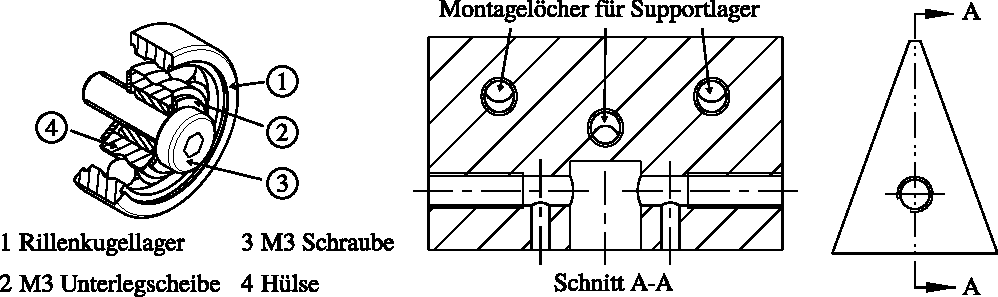
\includegraphics[]{./images/kugelsupport.pdf}
    \caption{Das Supportlager (links) und der Kunststoffsockel (rechts)}
    \label{fig:das_modifizierte_kugelsupport}
\end{figure}
%

Der Kohlebürstenhalter ist aus Messing, hat eine zylindrische Form und wird mit einem Blechhalter, welcher an der Seite des Supports angeschraubt wird, gelötet.
Die Kohlebürste Typ \textit{KK399} wurden von der Firma \textit{Schmidthammer} gekauft.
Dank dem hohen Kupferanteil (98\%) hat sie sehr geringen Kontaktwiderstand bzw. Eigenwiderstand.
Sie hat am Ende eine Kupferlitze und ist an anderen Seite mit Laufschräge zu versehen.
Leider ist die Laufschräge für diese Anwendung nicht geeignet und wurden flach geschliffen.
Die Kohlebürste wird von einer Feder (Typ \textit{LG860}) gegen der Lauffläche (Kugelaufnahme) gedrückt.
Abbildung \ref{fig:die_baugruppe_des_kohlebuerstenhalters} zeigt die Baugruppe des Kohlebürstenhalters.
% ----------------------------------------
% Fig: Blechhalter + Kohlebürstenhalter + Kohlebürsten + Feder
% ----------------------------------------
\begin{figure}[htb]
    \centering
    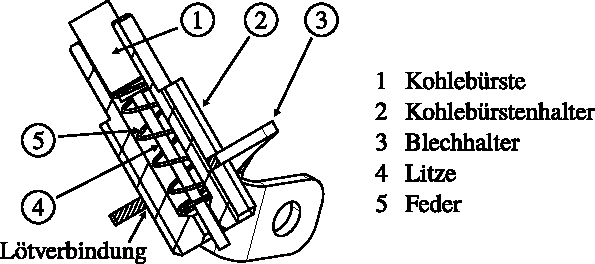
\includegraphics[]{./images/kohlebuerstenhalter_asm.pdf}
    \caption{Die Baugruppe des Kohlebürstenhalters}
    \label{fig:die_baugruppe_des_kohlebuerstenhalters}
\end{figure}
%

Um der elektrische Kontakt zwischen der Kugel und der Messprobe während der Versuche geringe Störungen zu halten, sind zwei Kohlebürsten für die Kugel zu versehen.
Abbildung \ref{fig:das_komplette_kugelsupports} zeigt das komplette Supports mit der neuen Kugelführung.
% ----------------------------------------
% Fig: Zusammenbau des gesamten Kugelsupports
% ----------------------------------------
\begin{figure}[htb]
    \centering
    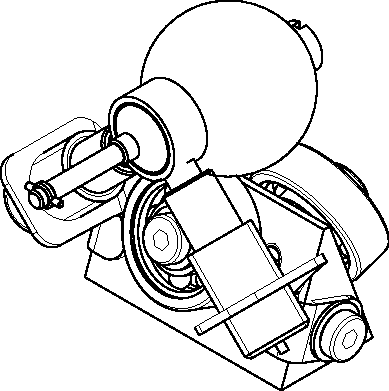
\includegraphics[]{./images/kugelsupport_full.pdf}
    \caption{Zusammenbau des neuen Supports mit der Kugel}
    \label{fig:das_komplette_kugelsupports}
\end{figure}
%

% ----------------------------------------
% Sec: Die Glasscheibebaugruppe
% ----------------------------------------
\section{Die Glasscheibebaugruppe}
\label{sec:die_glasscheibebaugruppe}

Um die elektrische Messung bei dem vorhandenen Prüfstand durchzuführen, müssen die folgende Maßnahmen gemacht werden:
\begin{itemize}
    \item Stromleitende Beschichtung für die Glasscheibe
    \item Isolierung der Glasscheibe mit dem gesamten Prüfsystem
    \item Elektrischer Zugang für die Messprobe zur Unterseite der Glasscheibe
\end{itemize}

Wie im vorherigen Kapitel \ref{chap:literaturforschung_der_experimentellen_technik_in_ehd_schmierung} schon erwähnt, ist es auch möglich, die Schmierfilmdickenmessung bei einer Chrom beschichteten Scheibe durch zu führen.
Allerdings es gibt folgende Probleme bei der klassischen Messmethode.
Ersten bietet dieses Verfahren eine niedrige Auflösung. Zweiten ist eine monochrom Lichtquelle notwendig, es fehlt bei dem vorhandenen Prüfstand diesen Apparat.
Nicht zuletzt ist das \textit{Ultra-Softwarepaket} von PCS nicht in der Lager solche Messung durchzuführen bzw. auszuwerten.
Letzten ist der Eigenwiderstand der Chromschicht wegen ihrer extrem dünnen Dicke sehr hoch (größer als $1 k\omega$) und unregelmäßig verteilt.
\label{chap:literaturforschung_der_experimentellen_technik_in_ehd_schmierung}
Das macht die optische und elektrische Messung bei der Chrom-Glasscheibe ungünstig.

Eine andere Option ist die \textit{Spacer-Layer-Scheibe} zu benutzen.
Da die Silikatschicht nicht Strom leitend ist, wird die Hälfte der Scheibe mit einer dickeren Chromschicht (c.a $300 nm$) beschichtet (Abbildung \ref{fig:die_neu_beschichtet_glassscheibe}).
Durch die Erhöhung der Beschichtung wird der Eigenwiderstand reduziert und auch besser auf der Oberfläche verteilt.
Die unbehandelte Hälfte kann man wie normal mit der \textit{Spacer-Layer-Methode} die Schmierfilmdicke bestimmen.
% ----------------------------------------
% Fig: Bild der neuen beschichteten Scheibe
% ----------------------------------------
\begin{figure}[htb]
    \centering
    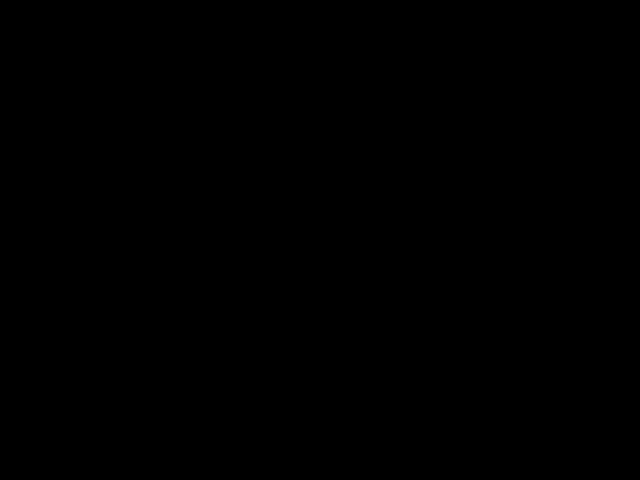
\includegraphics[width=4cm]{./images/blank_img.jpg}
    \caption{Die neu beschichtete Glasscheibe}
    \label{fig:die_neu_beschichtet_glassscheibe}
\end{figure}
%

Der nächste Schritt ist die behandelte Glasscheibe mit dem gesamten Testsystem isolieren.
Das erfolgt durch die Verwendung einer Kunststoff-Unterlegscheibe und einer Kunststoffhülse, die Unterseite der Scheibe mit der Welle des 1. Motors trennen (Abbildung \ref{fig:isolierung_der_glassscheibe})
% ----------------------------------------
% Fig: Isolierung der Scheibe
% ----------------------------------------
\begin{figure}[htb]
    \centering
    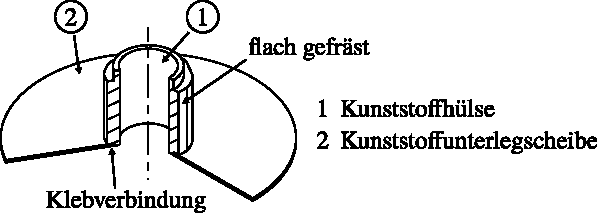
\includegraphics[]{./images/isolierung_der_scheibe.pdf}
    \caption{Isolierung der Glasscheibe}
    \label{fig:isolierung_der_glassscheibe}
\end{figure}
%

Beide Teile sind aus \textit{Polypropylen}, welcher bis $80 ^\circ C$ beständig ist und die Unterlegscheibe ist nur $0,5 mm$ dick.
Da die Lasteinheit nicht nur in die horizontale sondern auch in die vertikale Richtung sich bewegen kann, ist diese minimale Höheänderung der Glasscheibe kein Problem.
Die äußere Oberfläche der Hülse wurden an sechs Positionen flach gefräst. Die bilden sich mit der inneren Bohrung der Glasscheibe sechs Kanäle, die den Platz für die elektrische Verbindungen von Unterseite zur Oberseite der Scheibe schaffen.
Die Kunststoff-Unterlegscheibe wurde mit der Hülse mit dem \textit{Plastix} Klebe von Pattex geklebt, diese Verbindung ist gegen dem Wegrutschen der beiden Teilen während Betriebs zu sichern.

Um die elektrische Verbindung von der Unterseite der Scheibe nach oben zu bringen, werden sechs Kupferstreifen verwendet.
Sie werden auf der Kunststoff-Unterlegscheibe angeklebt und durch die sechs Kanäle (zwischen Hülse und Glasscheibe) nach oben geführt.
Dort werden sie bei der Montageposition zwischen der Oberkante der Hülse und einer Mitnehmerscheibe geklemmt und dadurch ist die elektrische Verbindung zwischen beiden Seite Scheibe hergestellt.
Die von oben geschraubt Sicherungsmutter sichert die ganze Baugruppe fest.
Die Abbildung \ref{fig:glasscheibebaugruppe} zeigt die ganze Baugruppe der Glasscheibe an.
% ----------------------------------------
% Fig: Glasscheibebaugruppe
% ----------------------------------------
\begin{figure}[htb]
    \centering
    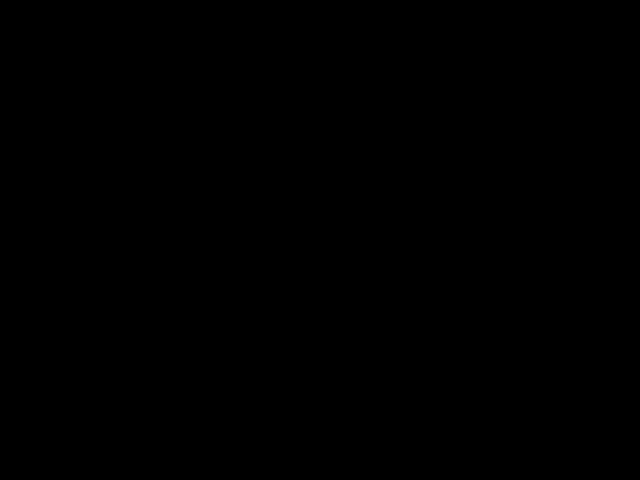
\includegraphics[width=4cm]{./images/blank_img.jpg}
    \caption{Glasscheibebaugruppe}
    \label{fig:glasscheibebaugruppe}
\end{figure}
%

% ----------------------------------------
% Sec: Konstruktion des Deckels
% ----------------------------------------
\section{Konstruktion des Deckels}
\label{sec:konstruktion_des_deckels}
